\subsection{Generic Geometry Settings\\通用几何设置}\label{subsec:vignettegeometry}

\begin{vigTcbKey}[][doc new=2016-04-22]{xmin}{=\meta{length}}{no default, initially |0pt|}
Sets the lower horizontal limit of a \refComLe{tcbvignette}.

设置 \refComLe{tcbvignette} 的下水平限制。
\end{vigTcbKey}

\begin{vigTcbKey}[][doc new=2016-04-22]{xmax}{=\meta{length}}{no default, initially |1cm|}
Sets the upper horizontal limit of a \refComLe{tcbvignette}.

设置 \refComLe{tcbvignette} 的上水平限制。
\end{vigTcbKey}

\begin{vigTcbKey}[][doc new=2016-04-22]{ymin}{=\meta{length}}{no default, initially |0pt|}
Sets the lower vertical limit of a \refComLe{tcbvignette}.

设置 \refComLe{tcbvignette} 的下垂直限制。
\end{vigTcbKey}

\begin{vigTcbKey}[][doc new=2016-04-22]{ymax}{=\meta{length}}{no default, initially |1cm|}
Sets the upper vertical limit of a \refComLe{tcbvignette}.

设置 \refComLe{tcbvignette} 的上垂直限制。
\end{vigTcbKey}


\begin{dispExample*}{sbs,righthand width=3cm,center lower}
\begin{tikzpicture}
  \fill [black!20] (0,0) rectangle (3,2);
  \path [pattern=checkerboard,pattern color=black!30]
    (0,0) rectangle (3,2);
  \tcbvignette{xmin=1cm,xmax=2.5cm,ymin=0.5cm,ymax=1.75cm}
\end{tikzpicture}
\end{dispExample*}


\begin{vigTcbKey}[][doc new=2016-04-22]{lower left corner}{=\meta{coordinates}}{style, initially |0,0|}
Sets the lower left corner of a \refComLe{tcbvignette}.
This style sets \refKeyLe{/tcb/vig/xmin} and \refKeyLe{/tcb/vig/ymin}.

设置一个\refComLe{tcbvignette}的左下角。 此样式设置\refKeyLe{/tcb/vig/xmin}和\refKeyLe{/tcb/vig/ymin}。
\end{vigTcbKey}

\begin{vigTcbKey}[][doc new=2016-04-22]{upper right corner}{=\meta{coordinates}}{style, initially |1,1|}
Sets the upper right corner of a \refComLe{tcbvignette}.
This style sets \refKeyLe{/tcb/vig/xmax} and \refKeyLe{/tcb/vig/ymax}.

设置一个\refComLe{tcbvignette}的右上角。 此样式设置\refKeyLe{/tcb/vig/xmax}和\refKeyLe{/tcb/vig/ymax}。
\end{vigTcbKey}


\begin{dispExample*}{sbs,righthand width=3cm,center lower}
\begin{tikzpicture}
  \fill [black!20] (0,0) rectangle (3,2);
  \path [pattern=checkerboard,pattern color=black!30]
    (0,0) rectangle (3,2);
  \tcbvignette{lower left corner={1,0.5},
               upper right corner={2.5,1.75}}
\end{tikzpicture}
\end{dispExample*}

\enlargethispage*{1cm}

\begin{vigTcbKey}[][doc new=2016-04-22]{inside node}{=\meta{name}}{style, initally unset}
Places the \refComLe{tcbvignette} inside the node with the given \meta{name}.
The outer limits of the \emph{vignette} are adapted to the node geometry.

将\refComLe{tcbvignette}放置在给定\meta{name}的节点内部。 \emph{vignette}的外部限制会根据节点几何形状进行调整。
\begin{dispExample*}{sbs,righthand width=3cm,center lower}
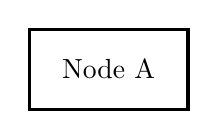
\begin{tikzpicture}
  \node[minimum width=2cm,minimum height=1cm] (A) {Node A};
  \tcbvignette{inside node=A}
  \draw[very thick] (A.south west) rectangle (A.north east);
\end{tikzpicture}
\end{dispExample*}
\end{vigTcbKey}

\begin{vigTcbKey}[][doc new=2016-04-22]{outside node}{=\meta{name}}{style, initally unset}
Places the \refComLe{tcbvignette} outside the node with the given \meta{name}.
The inner limits of the \emph{vignette} are adapted to the node geometry.

将\refComLe{tcbvignette}放置在给定\meta{name}的节点外部。内部\emph{vignette}的限制适应节点几何形状。
\begin{dispExample*}{sbs,righthand width=3cm,center lower}
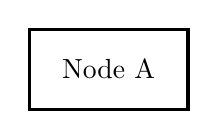
\begin{tikzpicture}
  \node[minimum width=2cm,minimum height=1cm] (A) {Node A};
  \tcbvignette{outside node=A}
  \draw[very thick] (A.south west) rectangle (A.north east);
\end{tikzpicture}
\end{dispExample*}
\end{vigTcbKey}


\begin{vigTcbKey}[][doc new=2016-04-22]{over node}{=\meta{name}}{style, initally unset}
Places the \refComLe{tcbvignette} over the node with the given \meta{name}.
The outer limits of the \emph{vignette} are adapted to the node geometry, but
are shifted to the outside by \refKeyLe{/tcb/vig/over node offset}.

将 \refComLe{tcbvignette} 放置在具有给定 \meta{name} 的节点上。 \emph{vignette} 的外部限制会根据节点几何形状进行调整,但是会向外移动 \refKeyLe{/tcb/vig/over node offset} 的偏移量。
\begin{dispExample*}{sbs,righthand width=3cm,center lower}
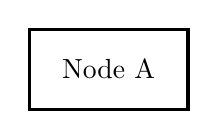
\begin{tikzpicture}
  \node[minimum width=2cm,minimum height=1cm] (A) {Node A};
  \tcbvignette{over node offset=1mm,over node=A}
  \draw[very thick] (A.south west) rectangle (A.north east);
\end{tikzpicture}
\end{dispExample*}
\end{vigTcbKey}

\begin{vigTcbKey}[][doc new=2016-04-22]{over node offset}{=\meta{length}}{no default, initially |0.1mm|}
Determines the shift value for \refKeyLe{/tcb/vig/over node}.
Note that \refKeyLe{/tcb/vig/over node offset} has to be set \emph{before}
\refKeyLe{/tcb/vig/over node} is used.

确定 \refKeyLe{/tcb/vig/over node} 的偏移值。 请注意,在使用 \refKeyLe{/tcb/vig/over node} 之前必须先设置 \refKeyLe{/tcb/vig/over node offset}。
\end{vigTcbKey}


\begin{vigTcbKey}[][doc new=2016-04-22]{north size}{=\meta{length}}{no default, initially |2mm|}
Sets the thickness of the north \emph{vignette} part.

设置北侧的vignette部分的厚度。
\begin{dispExample*}{sbs,righthand width=3cm,center lower}
\begin{tikzpicture}
  \tcbvignette{north size=4mm}
\end{tikzpicture}
\end{dispExample*}
\end{vigTcbKey}

\begin{vigTcbKey}[][doc new=2016-04-22]{south size}{=\meta{length}}{no default, initially |2mm|}
Sets the thickness of the south \emph{vignette} part.

设置南侧的vignette部分的厚度。
\begin{dispExample*}{sbs,righthand width=3cm,center lower}
\begin{tikzpicture}
  \tcbvignette{south size=4mm}
\end{tikzpicture}
\end{dispExample*}
\end{vigTcbKey}

\begin{vigTcbKey}[][doc new=2016-04-22]{east size}{=\meta{length}}{no default, initially |2mm|}
Sets the thickness of the east \emph{vignette} part.

设置东侧的vignette部分的厚度。
\begin{dispExample*}{sbs,righthand width=3cm,center lower}
\begin{tikzpicture}
  \tcbvignette{east size=4mm}
\end{tikzpicture}
\end{dispExample*}
\end{vigTcbKey}

\begin{vigTcbKey}[][doc new=2016-04-22]{west size}{=\meta{length}}{no default, initially |2mm|}
Sets the thickness of the west \emph{vignette} part.

设置西侧的vignette部分的厚度。
\begin{dispExample*}{sbs,righthand width=3cm,center lower}
\begin{tikzpicture}
  \tcbvignette{west size=4mm}
\end{tikzpicture}
\end{dispExample*}
\end{vigTcbKey}

% \clearpage

\begin{vigTcbKey}[][doc new=2016-04-22]{vertical size}{=\meta{length}}{style, initially |2mm|}
Sets \refKeyLe{/tcb/vig/north size} and \refKeyLe{/tcb/vig/south size},
to the given \meta{length}.

设置\refKeyLe{/tcb/vig/north size}和\refKeyLe{/tcb/vig/south size}为给定的\meta{length}。
\begin{dispExample*}{sbs,righthand width=3cm,center lower}
\begin{tikzpicture}
  \tcbvignette{vertical size=4mm}
\end{tikzpicture}
\end{dispExample*}
\end{vigTcbKey}

\begin{vigTcbKey}[][doc new=2016-04-22]{horizontal size}{=\meta{length}}{style, initially |2mm|}
Sets \refKeyLe{/tcb/vig/east size} and \refKeyLe{/tcb/vig/west size},
to the given \meta{length}.

设置\refKeyLe{/tcb/vig/east size}和\refKeyLe{/tcb/vig/west size}为给定的\meta{length}。
\begin{dispExample*}{sbs,righthand width=3cm,center lower}
\begin{tikzpicture}
  \tcbvignette{horizontal size=4mm}
\end{tikzpicture}
\end{dispExample*}
\end{vigTcbKey}


\begin{vigTcbKey}[][doc new=2016-04-22]{size}{=\meta{length}}{style, initially |2mm|}
Sets \refKeyLe{/tcb/vig/north size}, \refKeyLe{/tcb/vig/south size},
\refKeyLe{/tcb/vig/east size}, and \refKeyLe{/tcb/vig/west size} to the given \meta{length}.

将\refKeyLe{/tcb/vig/north size}、\refKeyLe{/tcb/vig/south size}、\refKeyLe{/tcb/vig/east size}和\refKeyLe{/tcb/vig/west size}设置为给定的\meta{length}。
\begin{dispExample*}{sbs,righthand width=3cm,center lower}
\begin{tikzpicture}
  \tcbvignette{size=4mm}
\end{tikzpicture}
\end{dispExample*}
\end{vigTcbKey}


\begin{marker}
\refKeyLe{/tcb/vig/north size}, \refKeyLe{/tcb/vig/south size}, etc. have to
be set \emph{before} \refKeyLe{/tcb/vig/outside node} is used.

\refKeyLe{/tcb/vig/north size},\refKeyLe{/tcb/vig/south size}等必须在使用\refKeyLe{/tcb/vig/outside node}之前进行设置。
\end{marker}